\documentclass{beamer}
%\documentclass[handout]{beamer}

\usetheme{Madrid}
\usecolortheme{spruce}
\setbeamercolor*{normal text}{fg=green!30!black,bg=green!5!white}
\usefonttheme{professionalfonts}
% TODO: Blaue Bullets => Grün.  Blaue Unterschrift "Abbildung" =>
% Grün.  Blautöne in Literaturverzeichnis => Grüntöne.

\usepackage[utf8]{inputenc}
\usepackage{csquotes}
\usepackage[ngerman]{babel}
\usepackage[backend=biber,style=numeric,sorting=nyvt]{biblatex}
\usepackage{tikz}
\usetikzlibrary{arrows,shapes,shapes.geometric,positioning}
\usepackage[export]{adjustbox}
\usepackage{pifont}
\usepackage{epigraph}

\newcommand{\clr}{olive}%
\newcommand{\cmark}{\ding{51}}%
\newcommand{\qmark}{\ding{51} / \ding{55}}%
\newcommand{\xmark}{\ding{55}}%
\newcommand{\COO}{\texorpdfstring{CO\textsubscript{2}}{CO 2}}%
\newcommand{\imply}{$\Rightarrow$}
\title[Kipppunkte]{
  Visualisierung der Hysterese\\
  von Kipppunkten}
\subtitle{Impulsvortrag mit anschließender Diskussion}
\author{Jürgen Reuter}
\institute[\tt{soundpaint.org}]{\tt{soundpaint.org}}
\date[LFF2023]{Letters for Future, 30.~September 2023}

\AtBeginSection[] {
  \begin{frame}[t]{Überblick}
    \tableofcontents[currentsection]
  \end{frame}
}

\addbibresource{../../bib/lff2023.bib}

%\listfiles % DEBUG: show package versions in log

\begin{document}

\tikzstyle{every picture}+=[remember picture]
\everymath{\displaystyle}

{\usebackgroundtemplate
  {\includegraphics[width=\paperwidth,height=\paperheight]
    {../images/title-image\_ultra-light.jpg}} \frame{\titlepage}}

%\begin{frame}[t]{Überblick}
%  \tableofcontents
%\end{frame}

%\section{Motivation \& Grundlagen}

\begin{frame}{Motivation \& Ziele I}
  \setlength{\epigraphwidth}{0.9\textwidth}
  \begin{epigraphs}
    \qitem{The likelihood and impacts of abrupt and/or irreversible
      changes in the climate system, including changes triggered when
      tipping points are reached, increase with further global warming
      {\em (high confidence)}.\vspace{1em}\\Die Wahrscheinlichkeit und
      die Auswirkungen abrupter und/oder unumkehrbarer Änderungen im
      Klimasystem, einschließlich solcher Änderungen, die ausgelöst
      werden, wenn Kipppunkte erreicht werden, nehmen mit der weiteren
      globalen Erwärmung zu {\em (hohe
        Sicherheit)}.}{\tiny\textit{IPCC Climate Change 2023 Synthesis
        Report (Summary for Policymakers), B3.2, Seite
        18\supercite{IPCC23}}}
  \end{epigraphs}
\end{frame}

\begin{frame}[t]{Motivation \& Ziele II}
  \begin{itemize}
  \item<2-> \color<2>{\clr} Was ist eine {\em Rückkopplung}
    (engl.\ {\em feedback})?
  \item<3-> \color<3>{\clr} Was ist ein {\em Kipppunkt} (engl.\ {\em
    tipping point})?
  \item<4-> \color<4>{\clr} Was ist ein {\em Kippelement} (engl.\ {\em
    tipping element})?
  \item<5-> \color<5>{\clr} Welche Beispiele gibt es?
  \item<6-> \color<6>{\clr} Was sind die grundsätzlichen Eigenschaften?
  \item<7-> \color<7>{\clr} Warum können die Auswirkungen {\em abrupt} sein?
  \item<8-> \color<8>{\clr} Warum können die Auswirkungen {\em
    irreversibel} sein?
  \item<9-> \color<9>{\clr} Welche weiteren Besonderheiten können
    auftreten?
  \end{itemize}
\end{frame}

\begin{frame}[fragile]{Rückkopplung I}
  % TODO: Bildchen ist suboptimal, weil es ein verstärkendes Element
  % im Signalweg darstellt, was ggf. an dieser Stelle so gar nicht
  % gegeben ist (vgl. z.B. Albedo-Beispiel); ggf. Verstärkung auch nur
  % im Rückkopplungszweig selbst.
  \tikz[remember picture, overlay] {
    \node[shift={(4cm, 2.5cm)}] at (current page.south west) (t1) {
      \tikzset{
        block/.style = {draw, rectangle, minimum height=1cm, minimum width=1cm},
        input/.style = {coordinate, node distance=2cm},
        output/.style = {coordinate, node distance=2cm},
        arrow/.style = {draw, -latex, node distance=2cm},
        pinstyle/.style = {pin edge={latex-, black, node distance=2cm}},
        sum/.style = {draw, circle, node distance=2cm}
      }
      \begin{tikzpicture}[auto, node distance=2.0cm,
          >=latex', every node/.style={scale=0.7}]
        \node<2-> [input, name=input] {};
        \node<2-> [sum, right of=input] (sum) {$+$};
        \node<2-> [isosceles triangle, draw, fill=yellow!20, minimum size=1cm, right of=sum] (function) {$f(t)$};
        \node<2-> [output, right=1.5cm of function] (output) {};
        \node<2-> [block, below of=function] (feedback) {$\beta$};
        \draw<2-> [draw,->] (input) -- node[label={[label distance=0.6cm]178:$Input$}] {} (sum);
        \draw<2-> [->] (sum) -- node {} (function);
        \draw<2-> [->] (function) -- node [name=y,label={[label distance=0.8cm]2:$Output$}] {}(output);
        \fill<2-> (y) [shift=(down:3pt)]circle (2pt);
        \draw<2-> [->] (y) |- node [above,pos=0.79] {} (feedback) ;
        \draw<2-> [->] (feedback) -| node[pos=0.99,shift=(down:10pt)] {$+$} node [near end] {} (sum);
      \end{tikzpicture}
    }
  }
  \vspace{-3.0cm}\\
  \begin{itemize}
  \item<2-> \color<2>{\clr} {\em Mitkopplung} oder {\em positive} Rückkopplung
    \begin{itemize}
    \item<3-> \color<3>{\clr} Ggf.\ aufschaukelnd verstärkende Wirkung
    \item<4-> \color<4>{\clr} Beispiele:
      \begin{itemize}
      \item<5-> \color<5>{\clr} „Pfeifendes“ Mikro
      \item<6-> \color<6>{\clr} Explosion
      \item<7-> \color<7>{\clr} Lawine
      \item<8-> \color<8>{\clr} Laser
      \item<9-> \color<9>{\clr} Zinseszinsen
      \end{itemize}
    \end{itemize}
  \end{itemize}
\end{frame}

\begin{frame}{Rückkopplung II}
  % TODO: Bildchen ist suboptimal, weil es ein verstärkendes Element
  % im Signalweg darstellt, was ggf. an dieser Stelle so gar nicht
  % gegeben ist (vgl. z.B. Albedo-Beispiel); ggf. Verstärkung auch nur
  % im Rückkopplungszweig selbst.
  \tikz[remember picture, overlay] {
    \node[shift={(4cm, 2.5cm)}] at (current page.south west) (t1) {
      \tikzset{
        block/.style = {draw, rectangle, minimum height=1cm, minimum width=1cm},
        input/.style = {coordinate, node distance=2cm},
        output/.style = {coordinate, node distance=2cm},
        arrow/.style = {draw, -latex, node distance=2cm},
        pinstyle/.style = {pin edge={latex-, black, node distance=2cm}},
        sum/.style = {draw, circle, node distance=2cm}
      }
      \begin{tikzpicture}[auto, node distance=2.0cm,
          >=latex', every node/.style={scale=0.7}]
        \node<2-> [input, name=input] {};
        \node<2-> [sum, right of=input] (sum) {$+$};
        \node<2-> [isosceles triangle, draw, fill=yellow!20, minimum size=1cm, right of=sum] (function) {$f(t)$};
        \node<2-> [output, right=1.5cm of function] (output) {};
        \node<2-> [block, below of=function] (feedback) {$\beta$};
        \draw<2-> [draw,->] (input) -- node[label={[label distance=0.6cm]178:$Input$}] {} (sum);
        \draw<2-> [->] (sum) -- node {} (function);
        \draw<2-> [->] (function) -- node [name=y,label={[label distance=0.8cm]2:$Output$}] {}(output);
        \fill<2-> (y) [shift=(down:3pt)]circle (2pt);
        \draw<2-> [->] (y) |- node [above,pos=0.79] {} (feedback) ;
        \draw<2-> [->] (feedback) -| node[pos=0.99,shift=(down:10pt)] {$-$} node [near end] {} (sum);
      \end{tikzpicture}
    }
  }
  \vspace{-3.0cm}\\
  \begin{itemize}
  \item<2-> \color<2>{\clr} {\em Gegenkopplung} oder {\em negative}
    Rückkopplung
    \begin{itemize}
    \item<3-> \color<3>{\clr} Abschwächende, dämpfende Wirkung
    \item<4-> \color<4>{\clr} Beispiele:
      \begin{itemize}
      \item<5-> \color<5>{\clr} Technischer Regelkreis:
      \item<6->[] \color<6>{\clr} Temperaturregler / Thermostat
        (Kühlschrank, Heizung)
      \item<7->[] \color<7>{\clr} Spannungsregler / stabilisiertes
        Netzteil
      \item<8->[] \color<8>{\clr} Fliehkraftregler
      \item<9-> \color<9>{\clr} Noise Cancelling
      \item<10-> \color<10>{\clr} Schilddrüsenfunktion
      \item<11-> \color<11>{\clr} Angebot und Nachfrage
      \item<12-> \color<12>{\clr} Temperaturkompensation,
        Frequenzkompensation (Harrison H4)
      \item<13-> \color<13>{\clr} Autofokus (Flankendiskriminator)
      \end{itemize}
    \end{itemize}
  \end{itemize}
\end{frame}

\begin{frame}[t]{Kipppunkt}
  \tikz[remember picture, overlay] {
    \node[shift={(0.50cm, 0.50cm)}] at (current page.south west) (t2) {
      \begin{tikzpicture}[remember picture, overlay]
        \draw<2->[thick,->](0.0, 0.5) -- (10.5, 0.5);
        \draw<2->[thick,->](0.5, 0.0) -- (0.5, 2.5);
      \end{tikzpicture}
    };
    \node[shift={(0.50cm, 0.50cm)}] at (current page.south west) (t2) {
      \begin{tikzpicture}[remember picture, overlay]
        \draw<2-4>[thick,->](0.0, 0.5) -- (10.5, 0.5) node[anchor=north
          east] {\hspace{-0.2cm}\scriptsize Eingangswert};
        \draw<2-4>[thick,->](0.5, 0.0) -- (0.5, 2.5) node[anchor=south
          west] {\hspace{-0.2cm}\scriptsize Ausgangswert};
      \end{tikzpicture}
    };
    \node[shift={(0.50cm, 0.50cm)}] at (current page.south west) (t2) {
      \begin{tikzpicture}[remember picture, overlay]
        \draw<5-7>[thick,->](0.0, 0.5) -- (10.5, 0.5) node[anchor=north
          east] {\hspace{-0.2cm}\scriptsize Temperatur};
        \draw<5-7>[thick,->](0.5, 0.0) -- (0.5, 2.5) node[anchor=south
          west] {\hspace{-0.2cm}\scriptsize Schneebedeckung};
      \end{tikzpicture}
    };
    \node[shift={(0.50cm, 0.50cm)}] at (current page.south west) (t2) {
      \begin{tikzpicture}[remember picture, overlay]
        \draw<8>[thick,->](0.0, 0.5) -- (10.5, 0.5) node[anchor=north
          east] {\hspace{-0.2cm}\scriptsize Lage des Schwerpunktes};
        \draw<8>[thick,->](0.5, 0.0) -- (0.5, 2.5) node[anchor=south
          west] {\hspace{-0.2cm}\scriptsize Auslenkung};
      \end{tikzpicture}
    };
    \node[shift={(0.50cm, 0.50cm)}] at (current page.south west) (t2) {
      \begin{tikzpicture}[remember picture, overlay]
        \draw<9>[thick,->](0.0, 0.5) -- (10.5, 0.5) node[anchor=north
          east] {\hspace{-0.2cm}\scriptsize Verstärker Eingangsspannung};
        \draw<9>[thick,->](0.5, 0.0) -- (0.5, 2.5) node[anchor=south
          west] {\hspace{-0.2cm}\scriptsize Verstärker Ausgangsspannung};
      \end{tikzpicture}
    };
    \node[shift={(0.50cm, 0.50cm)}] at (current page.south west) (t2) {
      {\color<3>{\clr}
        \begin{tikzpicture}[remember picture, overlay]
          \draw<3->(5.25, 1.0) -- (5.75, 2.5);
        \end{tikzpicture}
      }
    };
    \node[shift={(0.50cm, 0.50cm)}] at (current page.south west) (t2) {
      {\color<6>{\clr}
        \begin{tikzpicture}[remember picture, overlay]
          \draw<6->(5.75, 2.5) -- (10.0, 2.5);
        \end{tikzpicture}
      }
    };
    \node[shift={(0.50cm, 0.50cm)}] at (current page.south west) (t2) {
      {\color<7>{\clr}
        \begin{tikzpicture}[remember picture, overlay]
          \draw<7->(1.0, 1.0) -- (5.25, 1.0);
        \end{tikzpicture}
      }
    }
  }
  \vspace{-0.8cm}\\
  \begin{itemize}
  \item<2-> \color<2>{\clr} Mitkopplung
    \begin{itemize}
    \item[]<3-> \color<3>{\clr} {\imply} hohe Verstärkung, steile
      Flanke
    \end{itemize}
  \item<4-> \color<4>{\clr} Sättigung: Ausgangsgröße ggf.\ begrenzt
    (physikal.\ Limit)
    \begin{itemize}
    \item<5-> \color<5>{\clr} Beispiel: Schneebedeckung in
      niederschlagsreichem Gebiet
      \begin{itemize}
      \item<6-> \color<6>{\clr} maximal 100\% Schneebedeckung
      \item<7-> \color<7>{\clr} minimal 0\% Schneebedeckung
      \end{itemize}
    \item<8-> \color<8>{\clr} Beispiel Wippe: Begrenzte Auslenkung
    \item<9-> \color<9>{\clr} Beispiel OpAmp: Ausgangsspannung
      innerhalb Versorgungsspannung
    \end{itemize}
    \item[]<10->{\color<10>{\clr} {\imply} Schwellwert in System mit
      zwei (oder mehr) Zuständen}
    \item[]<11->{\color<11>{\clr} {\imply} rascher Zustandswechsel bei
      Schwellwertüberschreitung ({\em Kipppunkt})}
  \end{itemize}
\end{frame}

\begin{frame}{Kipp{\em punkt}?}
  \tikz[remember picture, overlay] {
    \node[shift={(0.45cm, 0.50cm)}] at (current page.south west) (t1) {
      \begin{tikzpicture}[remember picture, overlay]
        \draw<2->[step=0.5cm,gray!30!white,very thin] (0.1, 0.1) grid (10.4, 3.9);
      \end{tikzpicture}
    }
  }
  \tikz[remember picture, overlay] {
    \node[shift={(0.50cm, 0.50cm)}] at (current page.south west) (t2) {
      \begin{tikzpicture}[remember picture, overlay]
        {\color<2>{\clr} \draw<2->[thick,->](0.0, 0.5) -- (10.5, 0.5)
          node[anchor=north west] {\hspace{-3.3cm}\scriptsize
            Eingangsgröße (Ursache)}; }
      \end{tikzpicture}
    }
  }
  \tikz[remember picture, overlay] {
    \node[shift={(0.50cm, 0.50cm)}] at (current page.south west) (t3) {
      {\color<3>{\clr}
        \begin{tikzpicture}[remember picture, overlay]
          \draw<3->[thick,->](0.5, 0.0) -- (0.5, 4.0)
          node[anchor=south west] {\hspace{-0.2cm}\scriptsize
            Ausgangsgröße (Wirkung)};
        \end{tikzpicture}
      }
    }
  }
  \tikz[remember picture, overlay] {
    \node[shift={(0.50cm, 0.50cm)}] at (current page.south west) (t4) {
      {\color<4>{\clr}
        \begin{tikzpicture}[remember picture, overlay]
          \draw<4->(1.0, 1.0) -- (5.5, 1.0)
          node[anchor=north]{\hspace{-5.0cm}\scriptsize Zustand 1};
        \end{tikzpicture}
      }
    }
  }
  \tikz[remember picture, overlay] {
    \node[shift={(0.50cm, 0.50cm)}] at (current page.south west) (t5) {
      {\color<5>{\clr}
        \begin{tikzpicture}[remember picture, overlay]
          \draw<5->(5.5, 3.5) -- (10.0, 3.5)
          node[anchor=south]{\hspace{-5.0cm}\scriptsize Zustand 2};
        \end{tikzpicture}
      }
    }
  }
  \tikz[remember picture, overlay] {
    \node[shift={(0.50cm, 0.50cm)}] at (current page.south west) (t6) {
      {\color<6>{\clr}
        \begin{tikzpicture}[remember picture, overlay]
          \draw<6->[dashed](5.5, 1.0) -- (5.5, 3.5);
        \end{tikzpicture}
      }
    }
  }
  \vspace{-3.5cm}\\
  Erstes, naives Modell: Einzelne abrupte Schwelle
  \begin{itemize}
    \item<2-> \color<2>{\clr} Eingehende Größe (z.B.\ Last auf Wippe,
      \COO-Gehalt der Luft)
    \item<3-> \color<3>{\clr} Ausgehende Größe (Neigung der Wippe,
      Erderwärmung)
    \item<4-> \color<4>{\clr} Zustand 1 (Neigung zu einer Seite,
      kälteres Klima)
    \item<5-> \color<5>{\clr} Zustand 2 (Neigung zur anderen Seite,
      wärmeres Klima)
    \item<6-> \color<6>{\clr} Abrupter Zustandswechsel ({\em
      Kipppunkt})
  \end{itemize}
\end{frame}

% TODO:

% Gründe für eigentliche Hysterese: (1) Rückkopplung, (2) "Kosten" für
% Zustandswechsel (Reibung / Widerstand im Kippbereich).

% Gründe für verzögertes Erreichen des Hysterese-Bereichs durch Puffer
% / Speicher: (1) Beispiel Albedo: Dicke der Schneeschicht,
% d.h. Puffer bis Schnee geschmolzen ist.  (2) Beispiel
% Sauerstoffkatastrophe: Zunächst die im Meerwasser gelösten Ionen
% oxidiert; erst dann Anstieg O₂.

% Beispiel präparierte Wippe: Versteckte Kugel als Gewicht mit
% nicht-fixem Ort ist Kombi aus eigentlicher Hysterese (Rückkopplung)
% plus Verzögerung (Ort der Kugel als Speicherung).

\begin{frame}{Kipp{\em element}!}
  \tikz[remember picture, overlay] {
    \node[shift={(0.45cm, 0.50cm)}] at (current page.south west) (t1) {
      \begin{tikzpicture}[remember picture, overlay]
        \draw<1->[step=0.5cm,gray!30!white,very thin] (0.1, 0.1) grid (10.4, 3.9);
      \end{tikzpicture}
    }
  }
  \tikz[remember picture, overlay] {
    \node[shift={(0.50cm, 0.50cm)}] at (current page.south west) (t2) {
      \begin{tikzpicture}[remember picture, overlay]
        \draw<1->[thick,->](0.0, 0.5) -- (10.5, 0.5) node[anchor=north
          west] {\hspace{-3.3cm}\scriptsize Eingangsgröße (Ursache)};
      \end{tikzpicture}
    }
  }
  \tikz[remember picture, overlay] {
    \node[shift={(0.45cm, 0.50cm)}] at (current page.south west) (t3) {
      \begin{tikzpicture}[remember picture, overlay]
        \draw<1->[thick,->](0.5, 0.0) -- (0.5, 4.0) node[anchor=south
          west] {\hspace{-0.2cm}\scriptsize Ausgangsgröße (Wirkung)};
      \end{tikzpicture}
    }
  }
  \tikz[remember picture, overlay] {
    \node[shift={(0.50cm, 0.50cm)}] at (current page.south west) (t4) {
      {\color<2>{\clr}
        \begin{tikzpicture}[remember picture, overlay]
          \draw<2->(1.0, 1.0) -- (6.0, 1.0)
          node[anchor=north]{\hspace{-5.0cm}\scriptsize Zustand 1};
        \end{tikzpicture}
      }
    }
  }
  \tikz[remember picture, overlay] {
    \node[shift={(0.50cm, 0.50cm)}] at (current page.south west) (t5) {
      {\color<3>{\clr}
        \begin{tikzpicture}[remember picture, overlay]
          \draw<3->(5.0, 3.5) -- (10.0, 3.5)
          node[anchor=south]{\hspace{-5.0cm}\scriptsize Zustand 2};
        \end{tikzpicture}
      }
    }
  }
  \tikz[remember picture, overlay] {
    \node[shift={(0.50cm, 0.50cm)}] at (current page.south west) (t6) {
      {\color<4>{\clr}
        \begin{tikzpicture}[remember picture, overlay]
          \draw<4->[thick,->] (6.0, 1.0) -- (7.5, 3.5);
        \end{tikzpicture}
      }
    }
  }
  \tikz[remember picture, overlay] {
    \node[shift={(0.50cm, 0.50cm)}] at (current page.south west) (t7) {
      {\color<5>{\clr}
        \begin{tikzpicture}[remember picture, overlay]
          \draw<5->[thick,<-](3.5, 1.0) -- (5.0, 3.5);
        \end{tikzpicture}
      }
    }
  }
  \tikz[remember picture, overlay] {
    \node[shift={(0.50cm, 0.50cm)}] at (current page.south west) (t8) {
      {\color<6>{\clr}
        \begin{tikzpicture}[remember picture, overlay]
          \draw<6->[thick,<->](4.25, 2.25) -- (6.75, 2.25)
          node[anchor=south east]{\hspace{-2.0cm}\scriptsize
            Hysterese};
        \end{tikzpicture}
      }
    }
  }
  \vspace{-3.5cm}\\
  Verfeinertes Modell: Hysterese
  \begin{itemize}
    \item<2-> \color<2>{\clr} Zustand 1 (Neigung zu einer Seite,
      kälteres Klima)
    \item<3-> \color<3>{\clr} Zustand 2 (Neigung zur anderen Seite,
      wärmeres Klima)
    \item<4-> \color<4>{\clr} Wechsel{\em bereich} Zustandsübergang 1
      {$\rightarrow$} 2
    \item<5-> \color<5>{\clr} Wechsel{\em bereich} Zustandsübergang 2
      {$\rightarrow$} 1
    \item<6-> \color<6>{\clr} {\imply} statt {\em Kipppunkt} besser:
      {\em Kippelement} mit {\em Hysterese}
  \end{itemize}
\end{frame}

%\begin{frame}[t]{Alternative Hystereseformen}
%  \begin{itemize}
%    \item<1-> \color<1>{\clr} Bisher: Form eines Parallelogramm
%    \item<2-> \color<2>{\clr} Realität: Keine Ecken
%    \item<3-> \color<3>{\clr} Sondern kurvige Form
%    \item<4-> \color<4>{\clr} Schleifenartige Form
%  \end{itemize}
%\end{frame}

%\begin{frame}[t]{Beispiele aus Physik, Technik und Natur, Wirtschaft}
%  Hysterese-Effekte bzw. -Anwendungen gibt es sehr häufig:
%  \begin{itemize}
%    \item<2-> \color<2>{\clr} Thermostat/Kühlschrank (vermeidet "Flackern")
%    \item<3-> \color<3>{\clr} Prellfreier Schwellwertschalter (Schmitt-Trigger)
%    \item<4-> \color<4>{\clr} Bistabile Kippschaltungen (z.B.\ Flipflop)
%    \item<5-> \color<5>{\clr} Ferromagnetische Magnetisierung
%    \item<6-> \color<6>{\clr} KI / Neuronen: Sigmoid-Aktivierung + Rückkopplung
%    \item<7-> \color<7>{\clr} Diverse ökonomische / soziale Prozesse
%    \item<8-> \color<8>{\clr} Schmelze weiß reflektierender Schneeflächen
%    \item<9-> \color<9>{\clr} Permafrostende: Freiwerdendes gebundenes Methangas
%  \end{itemize}
%\end{frame}

\begin{frame}{\glqq{}Point of No Return\grqq (\glqq{}PNR\grqq)?}
  % TODO: Vorwärtsreferenz auf präparierte Wippe in dieser Folie
  % eliminieren.  Zu diesem Zweck vielleicht eine Überblicksfolie über
  % alle in diesem Vortrag behandelte Modelle (nur Titel + Bildchen)
  % ziemlich zu Beginn des Vortrags einfügen?
  \tikz[remember picture, overlay] {
    \node[shift={(0.45cm, 0.50cm)}] at (current page.south west) (t1) {
      \begin{tikzpicture}[remember picture, overlay]
        \draw<1->[step=0.5cm,gray!30!white,very thin] (0.1, 0.1) grid (10.4, 3.9);
      \end{tikzpicture}
    }
  }
  \tikz[remember picture, overlay] {
    \node[shift={(0.50cm, 0.50cm)}] at (current page.south west) (t2) {
      \begin{tikzpicture}[remember picture, overlay]
        \draw<1->[thick,->](0.0, 0.5) -- (10.5, 0.5)
        node[anchor=north west] {\hspace{-0.8cm}\scriptsize \COO};
      \end{tikzpicture}
    }
  }
  \tikz[remember picture, overlay] {
    \node[shift={(0.45cm, 0.50cm)}] at (current page.south west) (t3) {
      \begin{tikzpicture}[remember picture, overlay]
        \draw<1->[thick,->](0.5, 0.0) -- (0.5, 4.0)
        node[anchor=south west] {\hspace{-0.3cm}\scriptsize Effekt};
      \end{tikzpicture}
    }
  }
  \tikz[remember picture, overlay] {
    \node[shift={(0.45cm, 0.50cm)}] at (current page.south west) (t4) {
      \begin{tikzpicture}[remember picture, overlay]
        \draw<1->(1.0, 1.0) -- (6.0, 1.0)
        node[anchor=north]{\hspace{-5.0cm}\scriptsize Zustand 1};
      \end{tikzpicture}
    }
  }
  \tikz[remember picture, overlay] {
    \node[shift={(0.45cm, 0.50cm)}] at (current page.south west) (t5) {
      \begin{tikzpicture}[remember picture, overlay]
        \draw<1->(5.0, 3.5) -- (10.0, 3.5)
        node[anchor=south]{\hspace{-5.0cm}\scriptsize Zustand 2};
      \end{tikzpicture}
    }
  }
  \tikz[remember picture, overlay] {
    \node[shift={(0.45cm, 0.50cm)}] at (current page.south west) (t6) {
      \begin{tikzpicture}[remember picture, overlay]
        \draw<1->[thick,->] (6.0, 1.0) -- (7.5, 3.5);
      \end{tikzpicture}
    }
  }
  \tikz[remember picture, overlay] {
    \node[shift={(0.45cm, 0.50cm)}] at (current page.south west) (t7) {
      \begin{tikzpicture}[remember picture, overlay]
        \draw<1->[thick,<-](3.5, 1.0) -- (5.0, 3.5);
      \end{tikzpicture}
    }
  }
  \tikz[remember picture, overlay] {
    \node[shift={(0.45cm, 0.50cm)}] at (current page.south west) (t8) {
      {\color<3>{red}
        \begin{tikzpicture}[remember picture, overlay]
          \draw<3->[thick,dashed] (7.5, 3.4) circle (0.2cm)
          node[anchor=north west]{\scriptsize ?};
        \end{tikzpicture}
      }
    }
  }
  \tikz[remember picture, overlay] {
    \node[shift={(0.45cm, 0.50cm)}] at (current page.south west) (t9) {
      {\color<3>{red}
        \begin{tikzpicture}[remember picture, overlay]
          \draw<3->[thick,dashed] (3.65, 1.1) circle (0.2cm)
          node[anchor=south west]{\scriptsize ?};
        \end{tikzpicture}
      }
    }
  }
  \tikz[remember picture, overlay] {
    \node[shift={(0.45cm, 0.50cm)}] at (current page.south west) (t10) {
      {\color<5>{red}
        \begin{tikzpicture}[remember picture, overlay]
          \draw<5->[thick,dashed] (6.8, 2.25) circle (0.2cm)
          node[anchor=south east]{\scriptsize ?};
        \end{tikzpicture}
      }
    }
  }
  \tikz[remember picture, overlay] {
    \node[shift={(0.45cm, 0.50cm)}] at (current page.south west) (t11) {
      {\color<5>{red}
        \begin{tikzpicture}[remember picture, overlay]
          \draw<5->[thick,dashed] (4.3, 2.25) circle (0.2cm)
          node[anchor=south east]{\scriptsize ?};
        \end{tikzpicture}
      }
    }
  }
  \vspace{-3.4cm}\\
  Ab wann geht es realistischerweise nicht mehr zurück?
  \begin{itemize}
    \item<2-> \color<2>{\clr} Im Modell
      \begin{itemize}
        \item<3-> \color<3>{\clr} Bei Verlassen des Hysteresebereichs?
      \end{itemize}
    \item<4-> \color<4>{\clr} In Realität, Beispiel präparierte Wippe
      mit Kugel
      \begin{itemize}
        \item<5-> \color<5>{\clr} Ggf.\ deutlich früher?
        \item<6-> \color<6>{\clr} Zusatzherausforderung der trägen Kugel
        \item<7-> \color<7>{\clr} Umkehrung der Rollrichtung der Kugel
        \item<8-> \color<8>{\clr} Ist-Geschwindigkeit der
          beschleunigten Kugel einrechnen
        \item[]<9-> \color<9>{\clr} \imply{} Gleichgewicht reicht
          nicht zum Stoppen
      \end{itemize}
  \end{itemize}
\end{frame}

%\section{Fallbeispiele mit Analyse \& Bewertung}

\begin{frame}[t]{Beispiel Klimakipppunkte}
  nach Schellnhuber, Stand 2008\supercite{Wikipedia20a,Maeder08}
  \begin{itemize}
    \item<2-> \color<2>{\clr} Abschmelzen des sommerlichen arktischen
      Meereises
    \item<3-> \color<3>{\clr} Abschmelzen des Grönländischen
      Eisschildes
    \item<4-> \color<4>{\clr} Abschmelzen des Westantarktischen
      Eisschildes
    \item<5-> \color<5>{\clr} Erlahmen der atlantischen thermohalinen
      Zirkulation
    \item<6-> \color<6>{\clr} Veränderung der El Niño-Southern
      Oscillation (ENSO)
    \item<7-> \color<7>{\clr} Zusammenbruch des indischen
      Sommermonsuns
    \item<8-> \color<8>{\clr} Veränderungen im Westafrikanischen
      Monsunsystem mit Auswirkungen auf Sahara und Sahelzone
    \item<9-> \color<9>{\clr} Entwaldung des tropischen Regenwaldes
    \item<10-> \color<10>{\clr} Rückgang borealer Wälder
  \end{itemize}
\end{frame}

% TODO: Ggf. Erkenntnisse über zusätzliche, erst später entdeckte
% Kippelemente auf neuer Folie ergänzen.

\begin{frame}{Beispiel: Albedo von Schneeflächen}
  % TODO: Pfeilspitzen in den Boden sollten gleiche Länge haben.
  % Pfeile statt mit gerader Linien besser mit geschlängelten Linien.
  % Ggf. Pufferaspekt der (dickeren) Schneedecke einzeichnen und
  % ansprechen.
  \tikz[remember picture, overlay] {
    \node[shift={(0.50cm, 0.50cm)}] at (current page.south west) (t1) {
      \begin{tikzpicture}[remember picture, overlay]
        \fill<1->(0.5, 0.5) -- (10.5, 0.5) -- (0.5, 3.0) -- (0.5, 0.5);
        \node[anchor=north west,shift={(+2cm,+0.5cm)}] {\scriptsize Boden};
      \end{tikzpicture}
    }
  }
  \tikz[remember picture, overlay] {
    \node[shift={(0.50cm, 0.50cm)}] at (current page.south west) (t2) {
      \begin{tikzpicture}[remember picture, overlay]
        \draw<1->(0.5, 0.5) -- (10.5, 0.5) -- (10.5, 2.0) -- (0.5, 2.0) -- (0.5, 0.5);
        \node[anchor=north west,shift={(+8cm,+0.5cm)}] {\scriptsize Schnee};
      \end{tikzpicture}
    }
  }
  \tikz[remember picture, overlay] {
    \node[shift={(0.45cm, 0.50cm)}] at (current page.south west) (t3) {
      \begin{tikzpicture}[remember picture, overlay]
        \draw<1->[thick,->](5.0, 2.0) -- (5.0, 3.0);
        \draw<1->[thick,->](6.0, 2.0) -- (6.0, 3.0);
        \draw<1->[thick,->](7.0, 2.0) -- (7.0, 3.0);
        \draw<1->[thick,->](8.0, 2.0) -- (8.0, 3.0);
        \draw<1->[thick,->](9.0, 2.0) -- (9.0, 3.0);
        \draw<1->[thick,->](10.0, 2.0) -- (10.0, 3.0);
      \end{tikzpicture}
    }
  }
  \tikz[remember picture, overlay] {
    \node[shift={(0.45cm, 0.50cm)}] at (current page.south west) (t4) {
      \begin{tikzpicture}[remember picture, overlay]
        \draw<1->[thick,<-,white](1.0, 1.0) -- (1.0, 3.0);
        \draw<1->[thick,<-,white](2.0, 1.0) -- (2.0, 3.0);
        \draw<1->[thick,<-,white](3.0, 1.0) -- (3.0, 3.0);
        \draw<1->[thick,<-,white](4.0, 1.0) -- (4.0, 3.0);
      \end{tikzpicture}
    }
  }
  \vspace{-2.8cm}\\
  {\small Albedo: Rückstrahlvermögen diffus reflektierender Oberflächen}
  \begin{itemize}
    \item<2-> \color<2>{\clr} Zustand 1: Schneedecke vorhanden
    \item<3->[] \color<3>{\clr} \imply{} Schnee reflektiert Licht
    \item<4->[] \color<4>{\clr} \imply{} Kalter Boden
    \item<5->[] \color<5>{\clr} \imply{} Neuschnee bleibt liegen
      {$\leftarrow$} Mitkopplung!
    \item<6-> \color<6>{\clr} Zustand 2: Schneedecke weggeschmolzen
    \item<7->[] \color<7>{\clr} \imply{} Dunkler Boden absorbiert
      Licht
    \item<8->[] \color<8>{\clr} \imply{} Warmer Boden
    \item<9->[] \color<9>{\clr} \imply{} Neuschnee schmilzt weg
      {$\leftarrow$} Mitkopplung!
  \end{itemize}
\end{frame}

\begin{frame}{Beispiel mechanisches Modell: Wippe}
  \tikz[remember picture, overlay] {
    \node[shift={(0.50cm, 0.50cm)}] at (current page.south west) (t1) {
      \begin{tikzpicture}[remember picture, overlay]
        \node<2-> (seesaw) at (100.0pt, 55.0pt)
                  {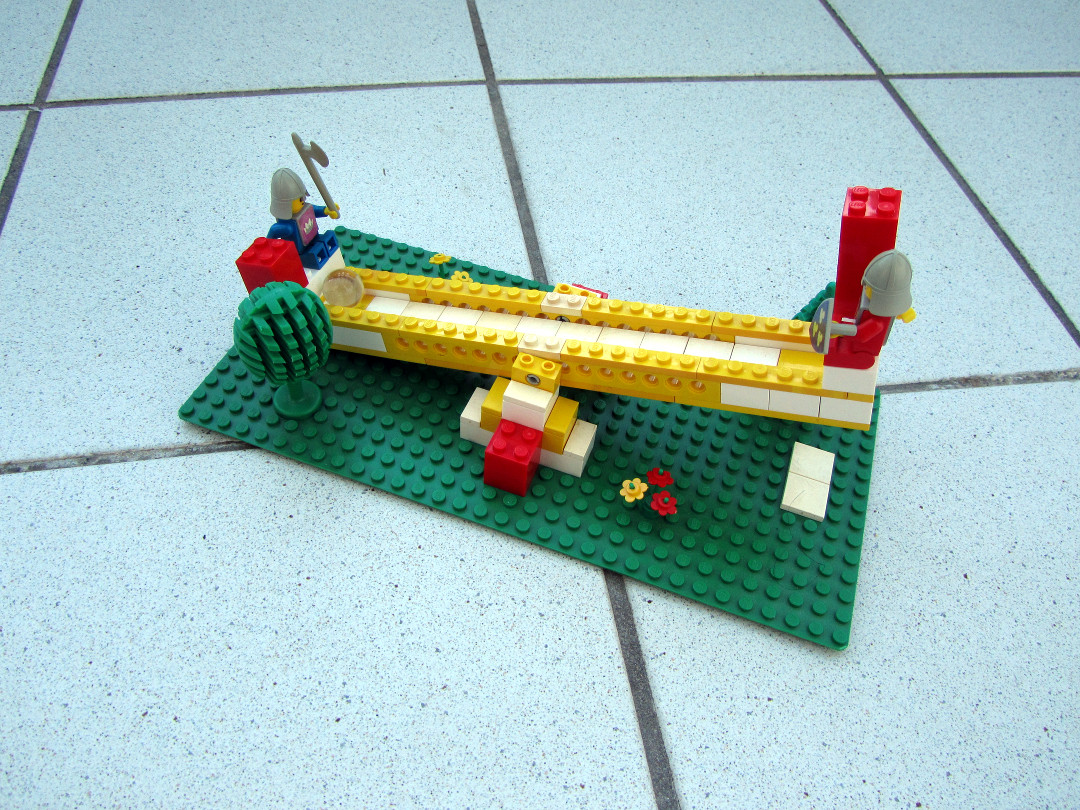
\includegraphics[width=200pt]{../images/seesaw.jpg}};
      \end{tikzpicture}
    }
  }
  \tikz[remember picture, overlay] {
    \node[shift={(0.50cm, 0.50cm)}] at (current page.south west) (t1) {
      {\color<3->{red}
        \begin{tikzpicture}[remember picture, overlay]
          \draw<3->[->,very thick](85.0pt, 135.0pt) -- (66.0pt, 80.0pt);
        \end{tikzpicture}
      }
    }
  }
  \vspace{-3.5cm}\\
  Präparierung mit Kugel
  \begin{itemize}
    \item<2-> \color<2>{\clr} Gewöhnliche Wippe: Hysterese vernachlässigbar
    \item<3-> \color<3>{\clr} Präparierte Wippe: Rollendes Gewicht im Balken
    \item<4-> \color<4>{\clr} Kugel rollt zum unteren Ende
    \item<5-> \color<5>{\clr} Hysterese durch Position der Kugel
  \end{itemize}
\end{frame}

\begin{frame}{Computersimulation der Wippe}
  \tikz[remember picture, overlay] {
    \node[shift={(0.50cm, 0.50cm)}] at (current page.south west) (t1) {
      \begin{tikzpicture}[remember picture, overlay]
        \node<2-> (seesaw) at (290.0pt, 145.0pt)
                  {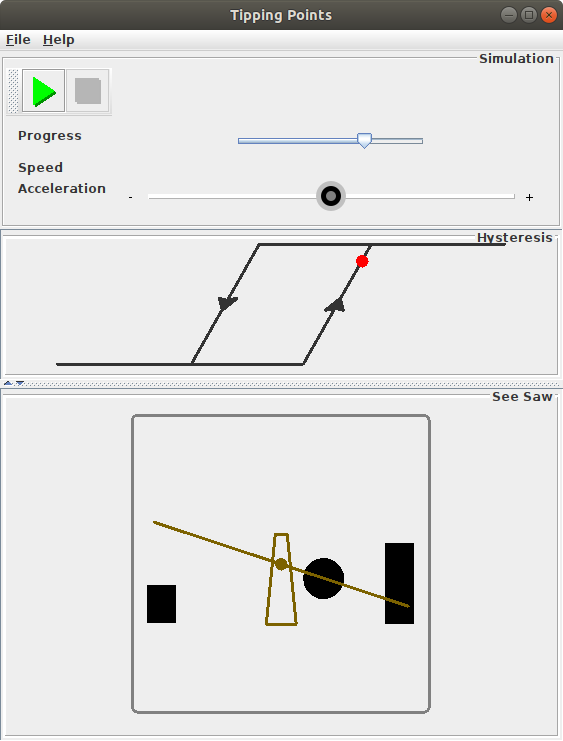
\includegraphics[width=100pt]{../images/simulation_v01.png}};
      \end{tikzpicture}
    }
  }
  \vspace{-1.5cm}\\
  Ein Modell ist ein {\em vereinfachtes} Abbild der Wirklichkeit.
  \begin{itemize}
    \item<2-> \color<2>{\clr} Nachbildung Wippe, rollende Kugel
    \item<3-> \color<3>{\clr} Vereinfachungen
      \begin{itemize}
        \item<4-> \color<4>{\clr} Konstant schnelles Rollen
        \item<5-> \color<5>{\clr} Simulationsumkehr vor Wendepunkt\\
        \item<6->[] \color<6>{\clr} \imply{} Aufwärtsrollen
      \end{itemize}
    \item<7-> \color<7>{\clr} Wirklichkeit deutlich komplexer
      \begin{itemize}
        \item<8-> \color<8>{\clr} Linear wachsende Geschwindigkeit der
          Kugel
        \item<9-> \color<9>{\clr} Richtungsumkehr: Kugel muss erst
          Abbremsen
        \item<10->[] \color<10>{\clr} \imply{} Umkehr zusätzlich
          erschwert
        \item<11-> \color<11>{\clr} Reibungskräfte am Drehpunkt
        \item<12-> \color<12>{\clr} Eigengewicht der Wippe
        \item<13-> \color<13>{\clr} Horizontale Position der Gewichte:
          Hebelgesetz!
        \item<14-> \color<14>{\clr} Äußere Einflüsse (Wind,
          Temperatur, Erschütterungen, $\dots$)
      \end{itemize}
  \end{itemize}
\end{frame}

\begin{frame}{Computersimulation der Wippe: Ergebnisse}
  \begin{itemize}
  \item<2-> \color<2>{\clr} Didaktisches, interaktives Spielzeug mit
    netter Grafik
  \item<3-> \color<3>{\clr} Für „ersten Kontakt“ mit Thematik nützlich
  \item<4-> \color<4>{\clr} Als reine Softwarelösung ohne spezielle
    Hardwarevoraussetzungen unkompliziert einsetzbar
  \item<4-> \color<4>{\clr} Nicht wirklich realitätsnah; primitives
    Modell mit sehr starken Vereinfachungen
  \end{itemize}
\end{frame}

% TODO: Blockdiagramm des elektronischen Modells

\begin{frame}{Elektronisches Modell}
  \tikz[remember picture, overlay] {
    \node[shift={(0.50cm, 0.00cm)}] at (current page.north west) (t1) {
      \begin{tikzpicture}[remember picture, overlay]
        \node (device-setup) at (0.5\textwidth, -3.00cm)
              {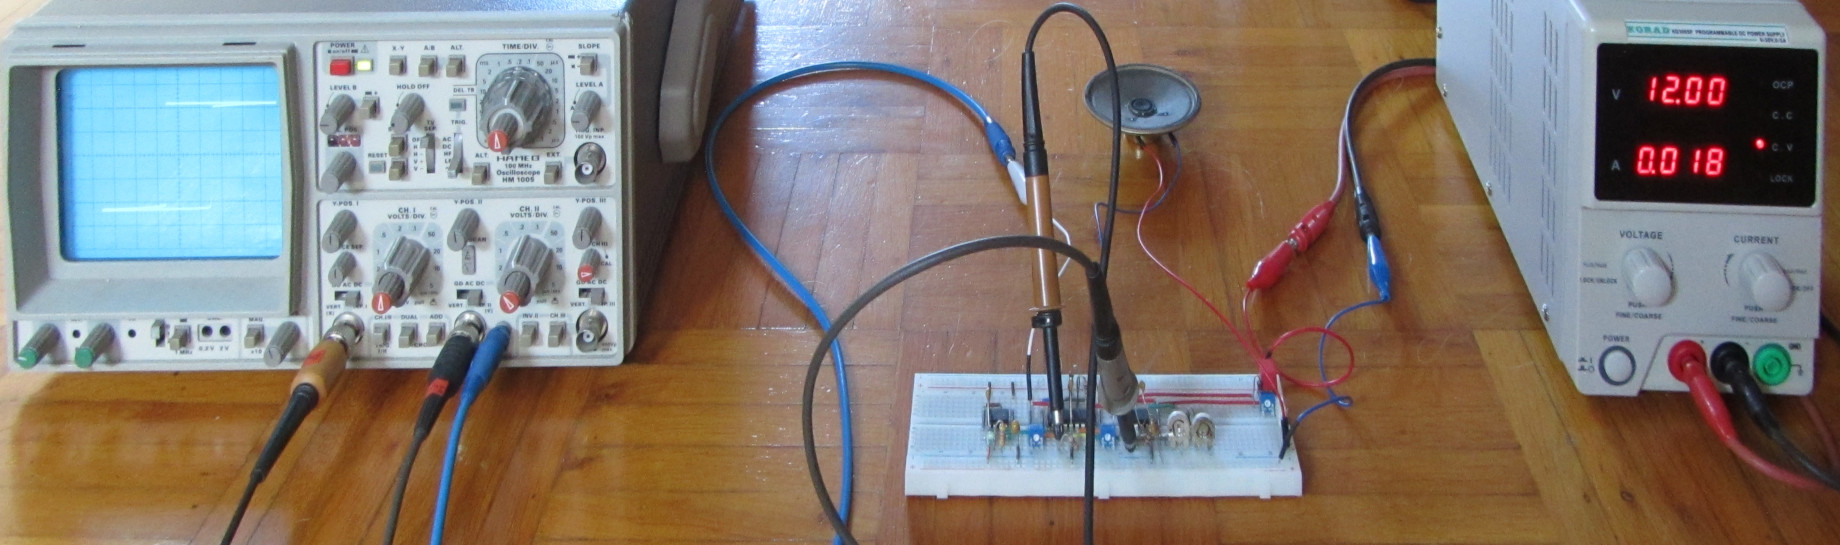
\includegraphics[width=0.9\textwidth]{../images/electronics-setup.jpg}};
        \draw<2>[draw=red,thick] (0.6cm, -1.5cm) rectangle ++(3.8cm, -2.1cm);
        \draw<3>[draw=red,thick] (5.9cm, -3.6cm) rectangle ++(2.4cm, -0.7cm);
        \draw<4>[draw=red,thick] (9.8cm, -1.5cm) rectangle ++(1.6cm, -2.3cm);
      \end{tikzpicture}
    }
  }
  \vspace{1.5cm}\\
  \begin{itemize}
  \item<2-> \color<2>{\clr} Oszilloskop für Visualisierung
  \item<3-> \color<3>{\clr} elektronisches Modell auf Breadboard
  \item<4-> \color<4>{\clr} Labornetzgerät, Spannungsversorgung 12V
  \end{itemize}
\end{frame}

\begin{frame}{Elektronisches Modell: Visualisierung}
  \begin{itemize}
    \item<2-> \color<2>{\clr} Oszilloskop zur Darstellung
    \item<3-> \color<3>{\clr} Betrieb im X-Y-Modus als {\em
      Kennlinienschreiber}
    \item<4-> \color<4>{\clr} Bildwiederholung für stehendes Bild
      notwendig
    \item<5->[] \color<5>{\clr} {\imply} Kippelement mit Oszillator
      periodisch durchwandern
    \item<6->[] \color<6>{\clr} {\imply} Dreieckschwingung erzeugen
      für Durchlaufen der X-Achse
    \item<7-> \color<7>{\clr} {\em Schmitt-Trigger} als eigentliches
      Kippelement
    \item<8-> \color<8>{\clr} Dreieck auf Eingang des Schmitt-Triggers
      legen
    \item<9-> \color<9>{\clr} Ausgang des Schmitt-Triggers: Y-Achse
  \end{itemize}
\end{frame}

\begin{frame}{Elektronisches Modell: Implementierung}
  % TODO: Bauteile in Abbildung mit rotem Rechteck einzeichnen
  \vspace{5.0cm} \tikz[remember picture, overlay] {
    {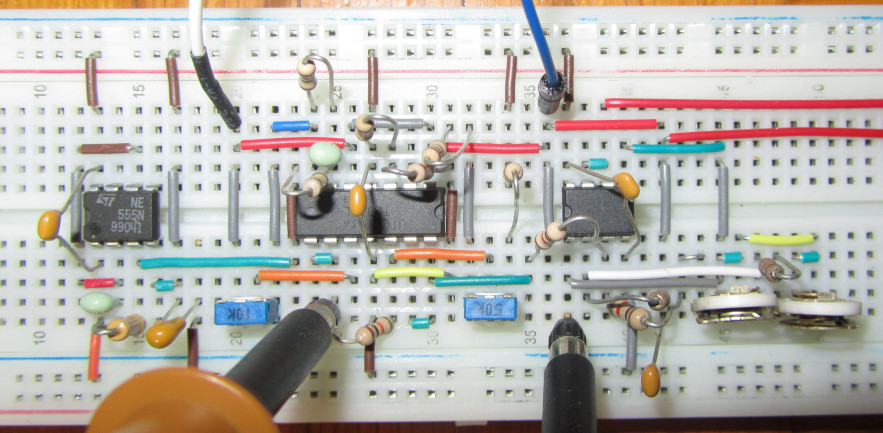
\includegraphics[width=0.9\paperwidth,center]
      {../images/breadboard.jpg}} }\\
  \begin{itemize}
  \item<2-> \color<2>{\clr} Implementierung auf Breadboard
  \item<3-> \color<3>{\clr} Oszillator mit Standardtimer
    \texttt{NE555}
  \item<4-> \color<4>{\clr} Integrator, Skalierung, Offset und
    Schmitt-Trigger mit Standard-OPV \texttt{TL07x}
  \end{itemize}
\end{frame}

\begin{frame}{Elektronisches Modell: Erzeugung Dreieckschwingung}
  \begin{itemize}
  \item<2-> \color<2>{\clr} Standard-Oszillatorschaltung
  \item<3-> \color<3>{\clr} Frequenz ca.\ 1,7kHz
  \item<4-> \color<4>{\clr} Signalaufbereitung
    \begin{itemize}
    \item<5-> \color<5>{\clr} Oszillation {\imply} nicht-lineare
      Ladekurve am Kondensator
    \item<6-> \color<6>{\clr} Schwellwertschalter {\imply}
      symmetrische Rechteckspannung
    \item<7-> \color<7>{\clr} Integrator {\imply} symmetrische
      Dreieckspannung
    \end{itemize}
  \item<8-> \color<8>{\clr} Frequenz der Oszillation im hörbaren
    Bereich
  \item<9-> \color<9>{\clr} Kalibrierung der Linearität (Klirrfaktor)
    auch per Lautsprecher möglich
  \end{itemize}
\end{frame}

\begin{frame}{Elektronisches Modell: Dreieckschwingung für X-Achse}
  \begin{figure}
    \centering
    \label{fig:charging_voltage}
    {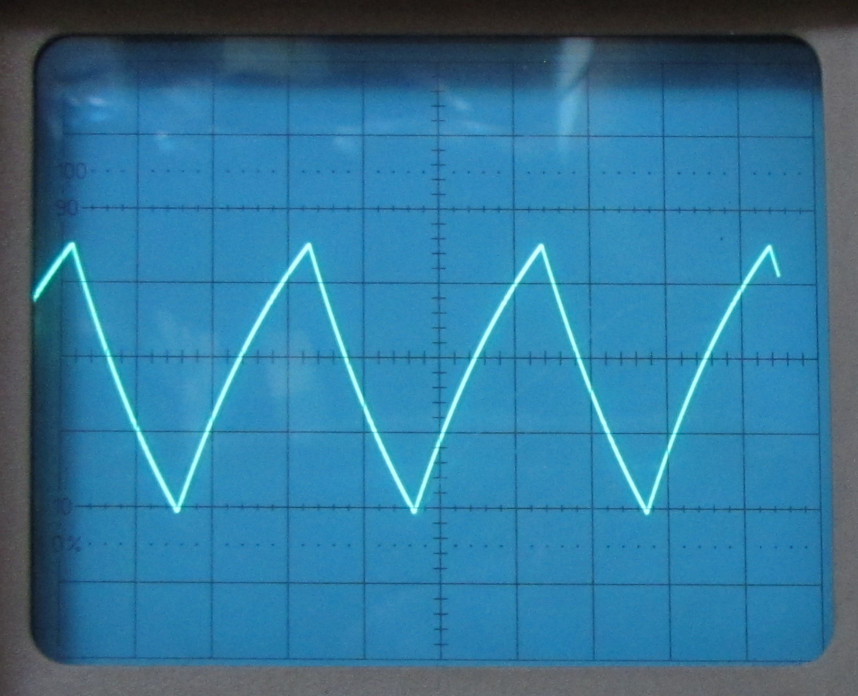
\includegraphics[width=0.5\paperwidth,center]
      {../images/charging-voltage.jpg}}
    \caption{Der Spannungsverlauf der Ladekurve am Kondensator des
      Oszillators kommt nur unzureichend der gewünschten
      Dreieckschwingung nahe.}
  \end{figure}
\end{frame}

\begin{frame}{Elektronisches Modell: Dreieckschwingung für X-Achse}
  \begin{figure}
    \centering
    \label{fig:sawtooth}
    {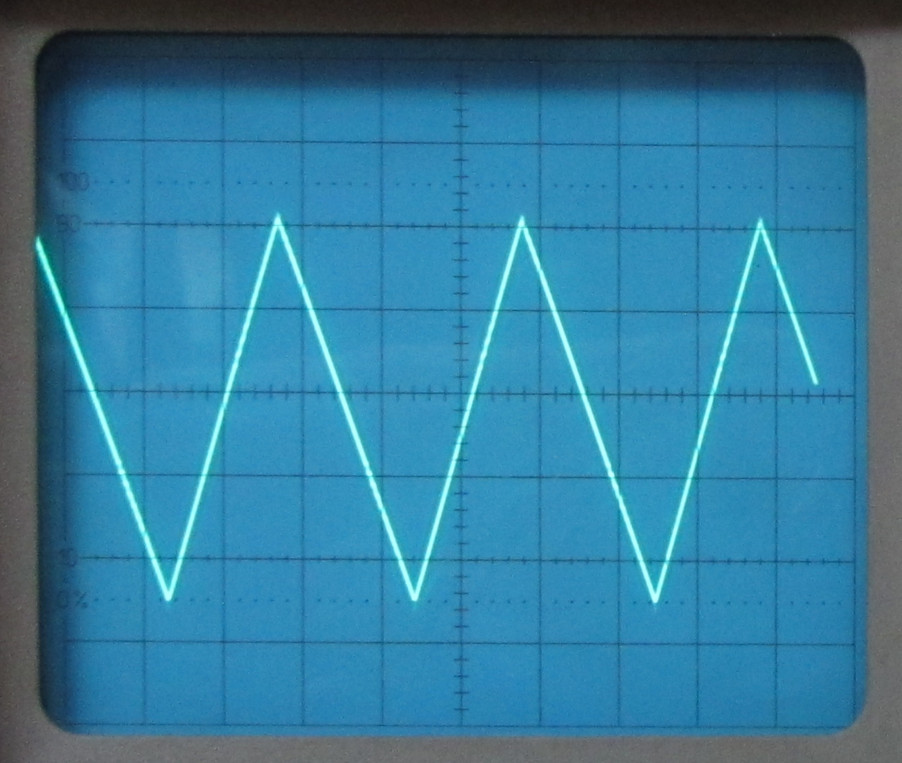
\includegraphics[width=0.5\paperwidth,center]
      {../images/sawtooth.jpg}}
    \caption{Der Spannungsverlauf der Ladekurve lässt sich per
      Schwellwertschalter in eine Rechteckschwingung und mit
      nachgeschaltetem Integrator in eine Dreieckschwingung hoher
      Genauigkeit wandeln.}
  \end{figure}
\end{frame}

\begin{frame}{Elektronisches Modell: Hysterese bei Volldurchlauf}
  \begin{figure}
    \centering
    \label{fig:hysteresis}
    {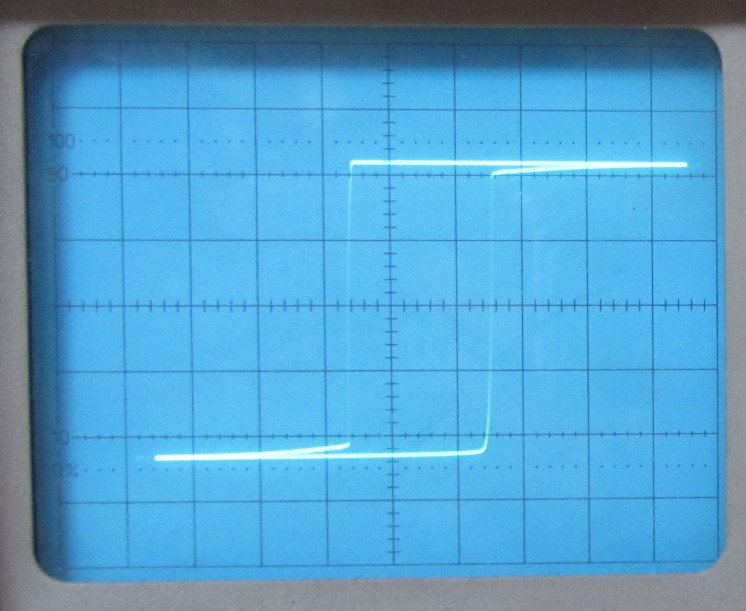
\includegraphics[width=0.5\paperwidth,center]
      {../images/hysteresis.jpg}}
    \caption{Für die Darstellung der Kennlinie wird die
      Dreieckspannung im X-Y-Modus des Oszilloskops als X-Wert
      verwendet und zugleich durch den Schmitt-Trigger geführt, dessen
      Ausgangspannung als Y-Wert dient.}
  \end{figure}
\end{frame}

\begin{frame}{Elektronisches Modell: Kehrtwende im Hysteresebereich}
  \begin{figure}
    \centering
    \label{fig:aborted_hysteresis}
    {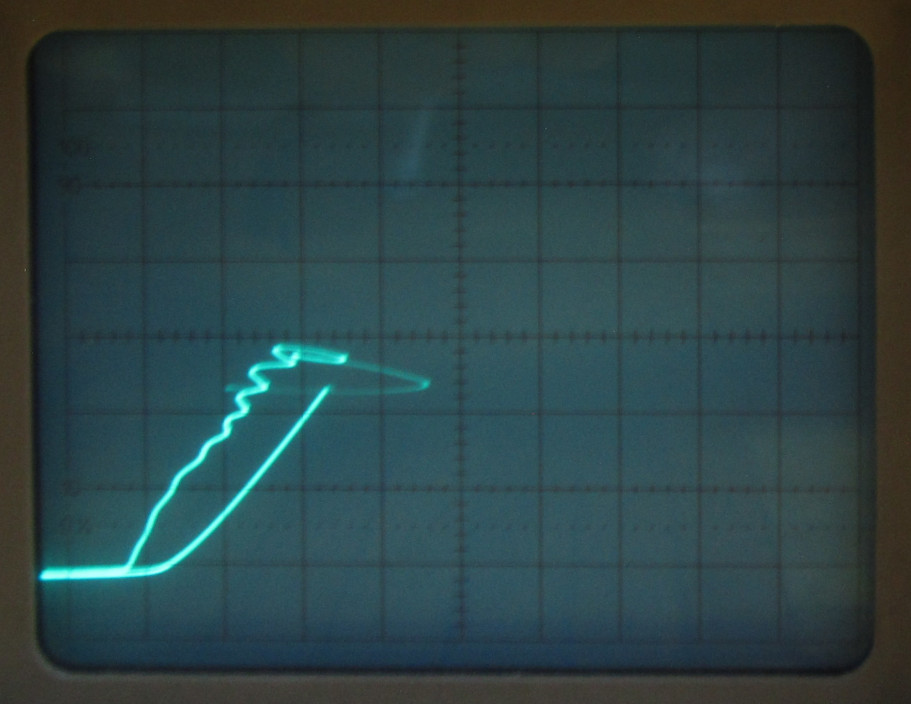
\includegraphics[width=0.5\paperwidth,center]
      {../images/aborted-hysteresis.jpg}}
    \caption{Wird die Dreieckschwingung so verschoben, dass der
      Hysteresebereich nicht mehr vollständig durchlaufen wird,
      sondern vorzeitig die Umkehr erfolgt, dann beginnt das System
      stark zu schwingen.  Die Hysterese kommt bereits bei Eintritt in
      den Hysteresebereich weitgehend zum Tragen.}
  \end{figure}
\end{frame}

% TODO: Linearer Übergang von Hysterese zu linearem Verstärker bei
% linearem Übergang von positiver zu negativer Rückkopplung.  Grafik /
% Oszi-Screenshot + Erläuterung.

\begin{frame}{Elektronisches Modell: Ergebnisse}
  \begin{itemize}
    \item<2-> \color<2>{\clr} Anders als die einfache
      Computersimulation „echtes“ Kippelement
    \item<3->[] \color<3>{\clr} {\imply} Potenzial, Effekte realer
      Kipppunkte besser herauszuarbeiten und abzubilden
    \item<4-> \color<4>{\clr} Parallelogramm-förmige Hysterese sehr
      gut visualisierbar
    \item<5-> \color<5>{\clr} Übergang zwischen Kippelement und
      Linearverstärker sehr gut visualisierbar
      \begin{itemize}
      \item<6-> \color<6>{\clr} Hohe Mitkopplung: Kippelement mit
        Hysterese
      \item<7-> \color<7>{\clr} Hohe Gegenkopplung: Lineare
        Verstärkung
      \end{itemize}
    \item<8-> \color<8>{\clr} Hysterese schlägt ggf.\ bereits bei
      Eintritt in Hysteresebereich voll durch
    \item<9-> \color<9>{\clr} Bei plötzlicher Kehrtwende im
      Hysteresebereich können ggf.\ starke Oszillationen auftreten
  \end{itemize}
\end{frame}

%\section{Ergebnisse \& Ausblick}

\begin{frame}[t]{Ergebnisse I}
  \begin{itemize}
    \item<2-> \color<2>{\clr} (Kleine) Hysterese praktisch immer
      vorhanden
      \begin{itemize}
      \item<3-> \color<3>{\clr} Wegen \glqq{}Kosten\grqq{} (Energie,
        Aufwand) für Zustandswechsel
      \item<4-> \color<4>{\clr} Durch Reibung, Wegstrecke,
        Abschmelzen, Einbringung, Entfernung, etc.
      \end{itemize}
    \item<5-> \color<5>{\clr} Größe der Hysterese abhängig von
      Mitkopplung \& Gegenkopplung
      \begin{itemize}
      \item<6-> \color<6>{\clr} Entscheidend für Irreversibilität
      \item<7-> \color<7>{\clr} Ggf.\ schwer zu bestimmen /
        abzuschätzen
      \end{itemize}
    \item<8-> \color<8>{\clr} Hysterese ggf.\ schon im
      Zustandsübergang voll wirksam
    \item<9-> \color<9>{\clr} veschiedene Hystereseformen und
      -dynamiken möglich
  \end{itemize}
\end{frame}

\begin{frame}[t]{Ergebnisse II}
  \begin{itemize}
    \item<2-> \color<2>{\clr} Modelle stets Vereinfachung der Realität
    \item<3-> \color<3>{\clr} Verschiedene Modelle betonen
      verschiedene Hysterese-Eigenschaften
      \begin{itemize}
      \item<4-> \color<4>{\clr} Wippe: ggf.\ Reibung, Hebelgesetz
      \item<5-> \color<5>{\clr} elektron.\ Modell: Oszillationen
      \end{itemize}
    \item<6-> \color<6>{\clr} Genauigkeit / Aussagekraft je Modell
      abhängig von Detaillierungsgrad
    \item<7-> \color<7>{\clr} Modell mit unerwartetem / überraschende Effekt
    \item<8-> \color<8>{\clr} Vielleicht nur „Problem“ des Modells
    \item<9-> \color<9>{\clr} Vielleicht aber Fingerzeig für bislang
      übersehene Eigenschaft
    \item<10-> \color<10>{\clr} Ggf.\ Anlass für weitere
      Untersuchungen
  \end{itemize}
\end{frame}

% TODO: Das Konzept des Kipppunkts ist im Ingenieurwesen seit
% Jahrhunderten (Jahrtausenden?) bekannt bzw. in Verwendung, aber
% dennoch nur erstaunlich oberflächlich erforscht.  Forschungsfragen:
% Klassifikation von Kipppunkten?  Formale Beschreibung der Klassen?
% Außer der Hysterese: Welche sonstigen Parameter zur Beschreibung /
% für Modellierung geeignet?

\begin{frame}[t]{Hysterese: Offene Fragen I}
  Für konkretes reales Kippelement
  \begin{itemize}
    \item<2-> \color<2>{\clr} Wie groß ist die Hysterese
      (z.B.\ Schneeflächen)?
      \begin{itemize}
        \item<3-> \color<3>{\clr} Jahre?
        \item<4-> \color<4>{\clr} Jahrzehnte?
      \end{itemize}
    \item<5-> \color<5>{\clr} Form der Hysterese?
      \begin{itemize}
        \item<6-> \color<6>{\clr} Z.B.\ Parallelogramm?
        \item<7-> \color<7>{\clr} Z.B.\ Schleife?
      \end{itemize}
    \item<8-> \color<8>{\clr} Wo ist der PNR?
    \item<9-> \color<9>{\clr} Gibt es weitere Einflüsse auf den PNR?
      \begin{itemize}
        \item<10-> \color<10>{\clr} Beispiel Wippe: beschleunigte Kugel
        \item<11-> \color<11>{\clr} Einfluss Luftfeuchtigkeit auf Niederschlag?
      \end{itemize}
    \item<12-> \color<12>{\clr} innere Variablen in Hysterese-Modell berücksichtigen
      \begin{itemize}
        \item<13-> \color<13>{\clr} z.B.\ Kugelposition bei der Wippe
        \item<14-> \color<14>{\clr} und Kugelgeschwindigkeit
      \end{itemize}
  \end{itemize}
\end{frame}

\begin{frame}[t]{Hysterese: Offene Fragen II}
  Für konkretes reales Kippelement
  \begin{itemize}
  \item<2-> \color<2>{\clr} Welches Modell kommt Realität am nächsten?
  \item<3-> \color<3>{\clr} In welchen Eigenschaften ist es realistisch?
  \item<4-> \color<4>{\clr} Worin unterscheidet es sich von Realität?
  \end{itemize}
\end{frame}

% bibliography
%\section{Literaturverweise}

\begin{frame}[t,allowframebreaks]{Literaturverweise}
  \nocite{Reuter20}
  \printbibliography
\end{frame}

\begin{frame}[t]
  \begin{center}
    \Huge{Diskussion eröffnet!}\\
    \vspace{1cm}
    \large{Gerne auch mit den Modellen „spielen“!}
  \end{center}
\end{frame}

% backup slides
%\section{Anhänge}

% TODO: Kurzeinführung OpAmp / Differenzverstärker

%\section*{Elektronisches Modell: Schaltpläne}

\begin{frame}[fragile]{Elektronisches Modell: Spannungsglättung und -verteilung}
  \begin{center}
    \includegraphics[width=0.75\textheight]{../schematics/voltage-supply.eps}
  \end{center}
\end{frame}

\begin{frame}[fragile]{Elektronisches Modell: Virtuelle Masse}
  \begin{center}
    \includegraphics[width=0.75\textheight]{../schematics/virtual-ground.eps}
  \end{center}
\end{frame}

\begin{frame}[fragile]{Elektronisches Modell: Rechteckschwingung ($\approx$ 1.7kHz)}
  \begin{center}
    \includegraphics[width=0.75\textheight]{../schematics/oscillator.eps}
  \end{center}
\end{frame}

\begin{frame}[fragile]{Elektronisches Modell: Wandlung Rechteck $\rightarrow$ Dreieck}
  \begin{center}
    \includegraphics[width=0.75\textheight]{../schematics/integrator.eps}
  \end{center}
\end{frame}

\begin{frame}[fragile]{Elektronisches Modell: Amplitudensteuerung}
  \begin{center}
    \includegraphics[width=0.75\textheight]{../schematics/osc-amplitude-ctrl.eps}
  \end{center}
\end{frame}

\begin{frame}[fragile]{Elektronisches Modell: Spannungspegelsteuerung}
  \begin{center}
    \includegraphics[width=0.75\textheight]{../schematics/osc-level-shift-ctrl.eps}
  \end{center}
\end{frame}

\begin{frame}[fragile]{Elektronisches Modell: Schmitt-Trigger}
  \begin{center}
    \includegraphics[width=0.75\textheight]{../schematics/schmitt-trigger.eps}
  \end{center}
\end{frame}

\begin{frame}[fragile]{Elektronisches Modell: Audio-Ausgang}
  \begin{center}
    \includegraphics[width=0.95\textheight]{../schematics/audio-out.eps}
  \end{center}
\end{frame}

\end{document}

%  Local Variables:
%    coding:utf-8
%    mode:LaTeX
%  End:
